
\subsection{实验环境与评价指标}

因为我们找不到任何拓扑跟踪数据SRLG链接,我们通过注入生成一个合成的数据集-ING SRLG进入华为拓扑跟踪发布。华为拓扑跟踪有7种不同的拓扑,具有不同的数目。节点、链路、链路权重(表示链路的延迟或其他参数)表一显示了基本的网络设置(编号)。这7个拓扑中的节点、链接)。基于华为的拓扑跟踪,我们随机生成SRLG组,使用SRLG图的注入数与SRLG边比(定义为SRLG边)(第3行和第4行)桌子。


As we could not find any topology trace data that contain SRLG links, we generate a synthesized data  set by injecting SRLG into a Huawei topology trace published. Huawei topology trace has $\TopoNum$ different topologies with various number of nodes, links, link weights (represent link's delay or other parameter). Table \ref{tab:AllSample} shows the basic network setting (number of nodes, links) in these $\TopoNum$ topologies. Based on huawei's topology trace, we randomly generate SRLG groups, with the number of SRLG graphs injected and the SRLG edge ratio (defined as $\frac{{No.SRLG \  {\rm{ }}edges}}{{Total \  {\rm{ }}No.edges}}$) shown on the 3rd and 4th rows of the table.



%The github website \cite{code} support complete experimental code and experimental topology data.}




\begin{table*}[tp]
\caption{$\TopoNum$ different topologies.}
  \centering
\footnotesize{  \begin{tabular}{*{18}{c}}
\toprule
Topology & 1 & 2 & 3 & 4 & 5 & 6& 7   \\
\midrule
Node    &     527&      521    &      521     &    2023             &     451     &     521     &     449       \\
Edge   &    4158 &  4052     &    4152      &   4142          &       2780   &      4052   &      2778    \\
%Graph density  & 1.5\% &    1.49\% &   1.52\%  &  0.1\%  &   0.10\% &   1.41\%  &  1.5\% &   1.38\%   \\
No.SRLG & 132 &  86   &  89  &  207        & 210  &  128  &   88    \\
SRLG edge ratio & 9.66\% & 6.16\% &   6.18\% &   14.94\%    &   22.55\%  &  9.65\% &   9.53\%     \\
\bottomrule
\end{tabular}
}

\label{tab:AllSample}
\end{table*}

为了进行性能比较,除了我们的方案(名为),我们还实现了另外四个SRLG-不相交。路由算法如下:

For performance comparisons, besides our scheme (named by \CI), we also implemented other four SRLG-disjoint routing algorithms as follows:

ILP:[19]中的工作旨在寻找SRLG-不相交的路径。通过ILP公式使总重量这两条路中的一条被最小化了。我们不知道其他的研究则寻找Min-Min SRLG-不相交路径。通过ILP公式。因此,在[19]之后,我们构造我们的Min-Min SRLG-不相交路由问题通过改变目标函数。2)iqcp:作为任意0−1整数线性规划,其中所有变量为0或1,ILP可表示为二次约束程序与ILP不同,我们还模拟了Min-Min SRLG- 不相交路由问题-整数二次约束规划(IQCP)[19]。3)KSP[23]:它在源和目标作为候选AP,然后一个接一个地测试它们要查看是否有相应的(不相交的)bp,直到我们发现了这样的BP。4)Cose[28]:当AP遇到陷阱问题时,Cose尝试进行简单而详尽的搜索,以找到SRLG。通过srlg集的AP无法找到的设置。不相交的BP 路径。基于SRLG集,它划分原问题并设计算法。若要搜索SRLG不相交路径对,请执行以下操作。

\begin{enumerate}
  \item ILP: The work in \cite{hu2003diverse}  aims to find SRLG-disjoint paths through an ILP formulation such that the total weight of the two paths are minimized. We are not aware that other studies look for the Min-Min SRLG-disjoint paths through ILP formulation. Therefore, following \cite{hu2003diverse}, we formulate  our Min-Min SRLG-disjoint routing problem by changing the objective function.
  \item IQCP: As any $0-1$ integer linear program where all variables are either 0 or 1,  ILP can be formulated as a quadratically constrained program. Different from ILP, we also model Min-Min SRLG-disjoint routing problem through the Integer Quadratic Constraints Program (IQCP) \cite{hu2003diverse}.
  \item KSP \cite{eppstein1998finding}: It finds the first $K$ shortest paths between the source and the destination as candidate APs, and then tests them one by one in the increasing order of their costs to see if it has a corresponding (disjoint) BP, until such a BP is found.
  \item CoSE \cite{rostami2007cose}: When an AP encounters a trap problem, CoSE tries a simple and exhaustive search to find a SRLG set that no AP going through the SRLG set can find the SRLG-disjoint BP path. Based on the SRLG set, it partitions the original problem  and designs an algorithm to search for the SRLG disjoint path pair.
\end{enumerate}
%\rev{As constraints of ILP equation for keeping linear calculation is $\sum\limits_{1\leq i \leq \chi} |\mathbb{R}_{r_i}|^2$ more than that of IQCP, ILP can be formulated as a quadratically constrained program so that reduce the quantity of constraints. As ILP}, we also model Min-Min SRLG-disjoint routing problem through the Integer Quadratic Constraints Program (IQCP) \rev{based on} \cite{hu2003diverse}.

前两者(ILP和IQCP)是基于整数程序的。模特。在我们的实现中,工具GUROBI 7.0[37]用于解决这两个整数问题。六次-性能指标用于评估不同的SRLG-不相交路由算法:路径权重:是路径中链接权重的总和。路径跳:路径中的跳数。运行时:平均毫秒数SRLG-不相交路径查找。算法加速比:给定两种情况下的计算时间不同的算法(算法1和算法2),表示为T1和T2,算法在算法2计算时间上的加速关于gal 1:s1−2=t1/t2。


核心加速比:并行程序的核心加速比[38]通常定义为SP=t1p,其中p是处理器内核和T1和Tp表示在1上的运行时间。核核和p核。效率:定义为[38]EP=SPP=t1PTP,它是典型的报告为范围内的百分比(0,1)。所有的模拟都是在linux服务器上运行的。使用Intel(R)Xeon(R)CPU E5-number00 2.00GHz(24核)和32.00GB内存。为了测量计算时间,我们在所有实现的算法中插入一个定时器。


The first two (ILP and IQCP) are based on integer program models. In our implementation, the tool GUROBI 7.0 \cite{optimization2012gurobi} is employed to resolve these two integer problems.  Six performance metrics are applied to evaluate the performance of different SRLG-disjoint routing algorithms:
%\begin{itemize}
%  \item \textbf{Path weight}: is the sum of the link weight in the path.
%  \item \textbf{Path hop}: the number of hops in the path
%  \item \textbf{Runtime}: the average number of milliseconds taken for SRLG-disjoint path finding.
%  \item \textbf{Algorithm speedup}: Given the computation time under two different  algorithms ($alg_1$ and $alg_2$), denoted as $T_1$ and $T_2$, the algorithm speedup in the computation time of the $alg_2$ with respect to the $alg_1$: ${S_{1 - 2}} = T_1/T_2$.
%  \item \textbf{Core speedup}: The core speedup \cite{bryant2003computer} of a parallel program is typically defined as $S_P=\frac{T_1}{T_p}$,
%where $p$ is the number of processor cores and $T_1$ and $T_p$ denote the running time on 1 core and $p$ cores, respectively.
%
%  \item \textbf{Efficiency}: is defined \cite{bryant2003computer} as $E_p=\frac{S_p}{p}=\frac{T_1}{pT_p}$,
%it is typically reported as a percentage in the range (0, 1].
%
%\end{itemize}

\textbf{Path weight}: is the sum of the link weight in the path.


 \textbf{Path hop}: the number of hops in the path.

\textbf{Runtime}: the average number of milliseconds taken for SRLG-disjoint path finding.


\textbf{Algorithm speedup}: Given the computation time under two different  algorithms ($alg_1$ and $alg_2$), denoted as $T_1$ and $T_2$, the algorithm speedup in the computation time of the $alg_2$ with respect to the $alg_1$: ${S_{1 - 2}} = T_1/T_2$.


 \textbf{Core speedup}: The core speedup \cite{grama2003introduction} of a parallel program is typically defined as $S_P=\frac{T_1}{T_p}$,
where $p$ is the number of processor cores and $T_1$ and $T_p$ denote the running time on 1 core and $p$ cores, respectively.


 \textbf{Efficiency}: is defined \cite{grama2003introduction} as $E_p=\frac{S_p}{p}=\frac{T_1}{pT_p}$,
it is typically reported as a percentage in the range (0, 1].




All simulations are run on a linux server, which is equipped with Intel(R) Xeon(R) CPU E5-2620 0 \@ 2.00GHz (24 Cores) and 32.00GB RAM. To measure the computation time, we insert a timer to all the implemented algorithms.


我们通过将SRLG注入到拓扑跟踪我们产生了两种SRLG。模拟,明星风格和非明星风格。光学网络,slg是明星风格,而在其他网络,如一个覆盖网络,SRLG可以是非星型的.每个SRLG组是通过随机选择2-5链接生成的.在五种SRLG不相交的路由算法,只有Cose和我们SCLS是并行算法。尽管ILP、IQCP和KSP不是并行算法,我们仍然在实现它们想给出我们的设计所获得的速度增益。我们以所有拓扑的归一化结果为最终结果。最小-最大归一化的仿真结果[39]为了节省空间。以获得更详细的模拟建立和仿真结果,我们的算法源代码。并可下载所合成的拓扑跟踪集。来自GitHub网站[40]


We generate the topology set by injecting SRLG into a topology trace. Two kinds of SRLG are generated in our simulation, the star-style and the non-star-style. In Optical Networks, SRLG is star-style, while in other networks such as an overlay network, SRLG can be non-star-style. Each SRLG group is generated by randomly selecting 2-5 links. Among the five SRLG disjoint routing algorithms, only CoSE and our SCLS are parallel algorithms. Although ILP, IQCP and KSP are not parallel algorithms, we still implement them as we want to present the speed gain obtained by our design. We take of the normalized results  of all topologies as the final simulation results according to min-max normalization \cite{tax2000feature} for the reason of space saving. For more detailed simulation setup and simulation result, the source codes of our algorithms and the synthesized topology trace sets can be downloaded from the github website \cite{code}




\subsection{Performance comparison}



\subsection{算法性能评估及比较}
根据第VII-B节的分析,在KSP下,COM-求第一条K最短路的计算复杂度是K(((E)V)log(V)),这将是很大的最坏的K=2 E。与分析一致,当我们使用7个拓扑运行ksp,没有仿真结果。在1小时内返回,而其他人则可以在11秒。计算时间长,使得ksp难以实现。在实践中使用。因此,我们不提供模拟。结果在KSP 下。


From the analysis in Section \ref{subsec:Complexity analysis}, under KSP, the computation complexity to find the first $K$ shortest paths is $K\times ((|\mathbb{E}|+|\mathbb{V}|)\times log(|\mathbb{V}|))$ , which would be large with the worst $K=2^{|\mathbb{E}|}$.
% where $K$ is the number of first  shortest paths that should be tested before finding the SRLG disjoint BP.}
 Consistent with the analysis, when we run KSP using the $\TopoNum$ topologies, no simulation results can be returned within 1 hour, while others can return results within 11 seconds. Long computation time makes KSP difficult to use in practice. Therefore, we do not provide the simulation results under KSP.

路径权重:图9显示AP、BP和AP和BP的总和。显然,所有的算法SCLS、Cose、ILP和IQCP实现了相同的AP。权重,但不同的BP权重因此不同的和权。AP和BP。因为所有算法都解决了相同的Min-MinSRLG-不相交的路由程序,尽管他们发现不同不相交的路径对,它们都能达到找到同样重量最小的AP。作为SCLS,Cose基于最短路径算法(如(Dijkstra),他们还发现BP路径具有相同的权重。然而,两个基于ILP的算法,ILP和iqcp,聚焦。如何最小化AP的权重但找到任何BPsrlg-与ap不相交,由这两条路径搜索到的bp路径。算法是不同的。2)路径跳:图10显示AP、BP和AP和BP之和因为所有算法的目标都是最小化SRLG- 不相交路径对的最小路径权重。在路径跳数中,它们具有相同的ap权重。(图9)尽管他们有不同的AP路径跳(图10)。

\subsubsection{Path Weight}
Fig.\ref{fig:normalization weitgh sum} shows the weight of AP, BP, and the sum of both AP and BP. Obviously, all implemented algorithms \CI, CoSE, ILP and IQCP achieve the same AP weight, but different BP weights thus different sum weights of AP and BP. As all the algorithms solve the same Min-Min SRLG-disjoint routing program, although they find different SRLG-disjoint path pairs, they can all achieve the goal of finding the  AP with the same least weight.
As \CI, CoSE find the  BP based on a shortest path algorithm (such as Dijkstra), they also find the BP path with the same weight. However, the two ILP-based algorithms, ILP and IQCP, focus on minimizing the weight of AP but find any BP that is SRLG-disjoint with AP, the BP paths searched by these two algorithms are different.

%\begin{figure*}[h]
%\begin{center}
%  % Requires \usepackage{graphicx}
%  \includegraphics[width=.25\textwidth]{franz/weight.eps}
%  \caption{Path weight}\label{fig:normalization weitgh sum}
%  \includegraphics[width=.25\textwidth]{franz/hop.eps}
%  \caption{Path hop}\label{fig:normalization hop}
%\end{center}
% \includegraphics[width=.25\textwidth]{franz/runtime}\\
%  \caption{Runtime}\label{fig:normalization runtime}
%\end{figure*}
\begin{figure}[tp]
\centering
\begin{minipage}[t]{0.45\linewidth}
\centering
\includegraphics[width=1.7in]{figures/weight}
\caption{Path weight}
\label{fig:normalization weitgh sum}
\end{minipage}
\hfill
\begin{minipage}[t]{0.45\linewidth}
\centering
\includegraphics[width=1.7in]{figures/hop}
\caption{Path hop}
\label{fig:normalization hop}
\end{minipage}
\end{figure}


\begin{figure*}[tp]
\centering
\begin{minipage}[t]{0.3\linewidth}
\centering
\includegraphics[width=2.25in]{figures/runtime}
\caption{Runtime}
\label{fig:normalization runtime}
\end{minipage}
\hfill
\begin{minipage}[t]{0.3\linewidth}
\centering
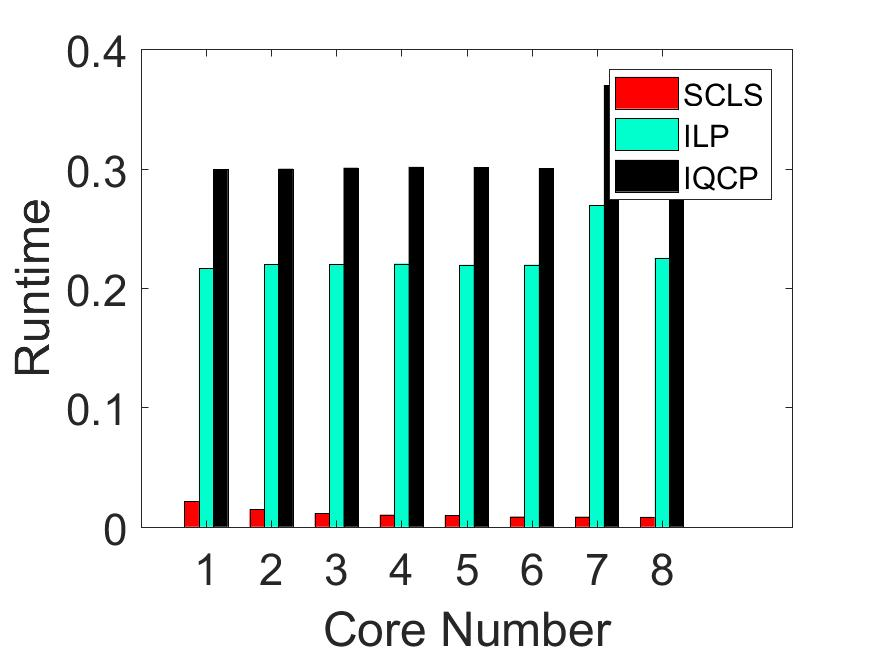
\includegraphics[width=2.25in]{figures/Runtime_noKSP_noCOSE}\\
  \caption{Runtime without CoSE}\label{fig:Runtime_noKSP_noCOSE}
\end{minipage}
\hfill
\begin{minipage}[t]{0.3\linewidth}
\centering
\includegraphics[width=2.25in]{figures/speedup}
\caption{Core speedup}
\label{fig:Speedup}
\end{minipage}
\end{figure*}


\begin{figure*}[tp]
\centering
\begin{minipage}[t]{0.3\linewidth}
\centering
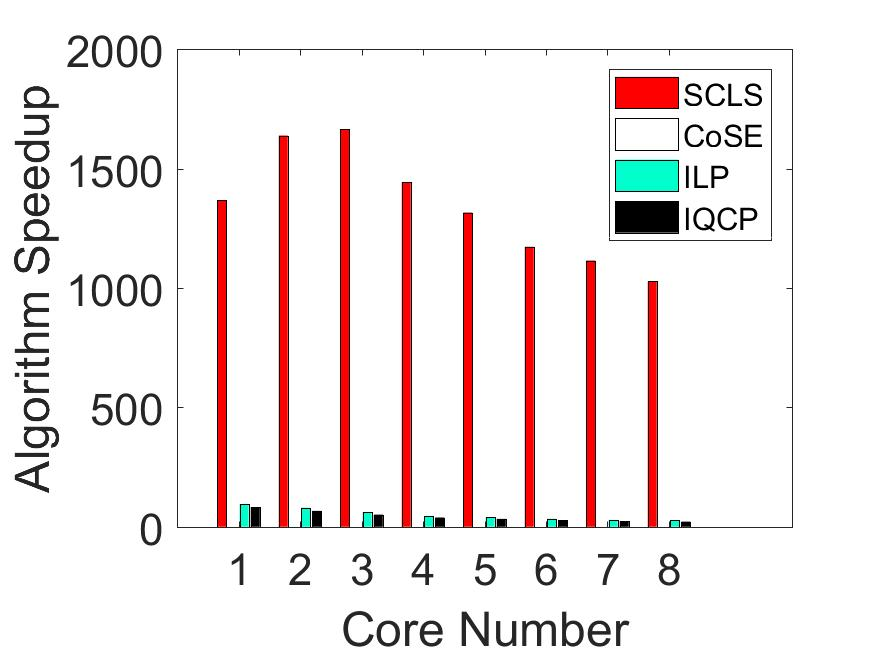
\includegraphics[width=2.25in]{figures/Multiple}
\caption{Algorithm speedup}
\label{fig:Multiple}
\end{minipage}
\hfill
\begin{minipage}[t]{0.3\linewidth}
\centering
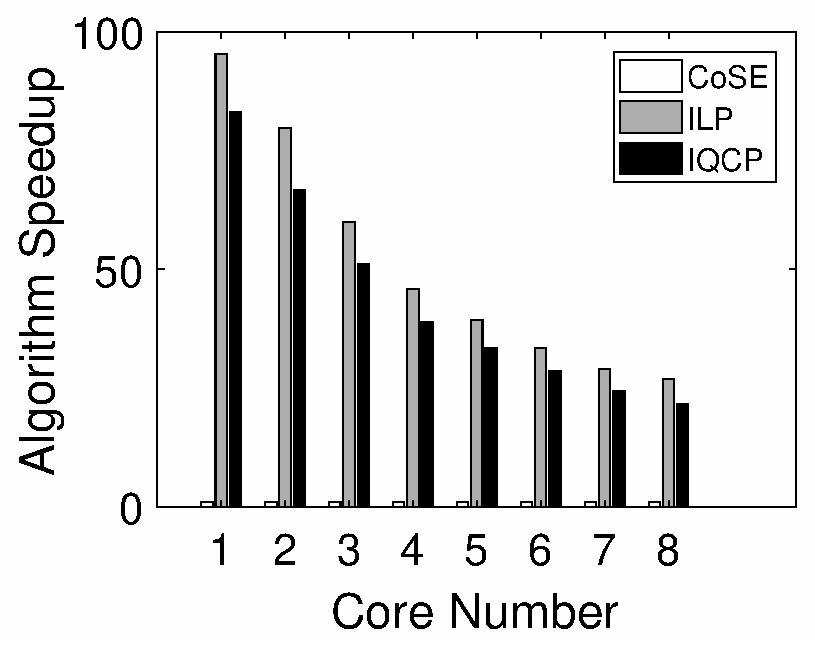
\includegraphics[width=2.25in]{figures/MultipleNoSCLS}
\caption{Algorithm speedup without SCLS}
\label{fig:MultipleNoSCLS}
\end{minipage}
\hfill
\begin{minipage}[t]{0.3\linewidth}
\centering
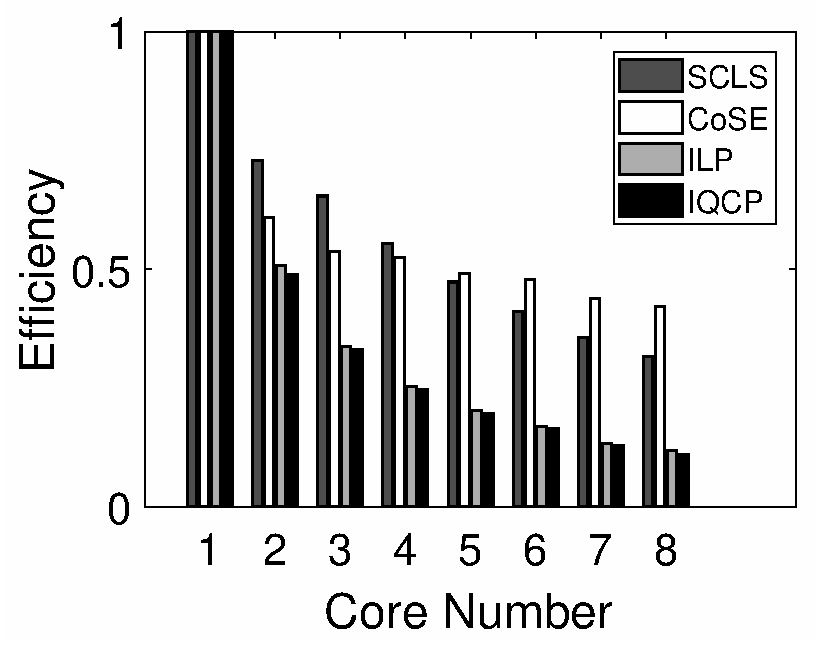
\includegraphics[width=2.25in]{figures/Efficiency}
 \caption{Efficiency}
 \label{fig:Efficiency}
\end{minipage}
\end{figure*}



\subsubsection{Path Hop}
Fig.\ref{fig:normalization hop} shows the path hop of AP, BP, and the sum of both AP and BP. As all algorithms target to minimize the least path weight of the SRLG-disjoint path pair instead of the number of path hops, they have the same AP weight (Fig.\ref{fig:normalization weitgh sum}) even though they have different AP path hops (Fig.\ref{fig:normalization hop}). Although the AP weights under all algorithms are smaller than the BP weights in Fig.\ref{fig:normalization weitgh sum}, in Fig.\ref{fig:normalization hop}, the AP hops may not always be fewer than the BP hops.

%\begin{figure}
%  \centering
%  % Requires \usepackage{graphicx}
%  \includegraphics[width=2.35in]{franz/hop}\\
%  \caption{Path hop}\label{fig:normalization hop}
%\end{figure}

尽管所有算法的AP权重都小于BP权重在图9中,在图10中,AP跳可能并不总是这样比英国石油公司的啤酒花还少。3)运行时:图11显示了不同运行时间下的运行时间算法通过改变CPU核的使用数量。如Cose下的运行时明显大于其他算法,以更清楚地显示其他算法的结果。算法,我们在图12中进一步绘制运行时结果因为ILP和IQCP不是并行算法,的不同数目下的这些算法的运行时。

\subsubsection{Runtime}
\label{subsubsec:Runtime}
Fig.\ref{fig:normalization runtime} shows the run time under different algorithms by varying the number of CPU cores utilized.
As the runtime under CoSE is significantly larger than that under other algorithms, to more clearly show the results of other algorithms, we further plot the runtime results in Fig.\ref{fig:Runtime_noKSP_noCOSE} by excluding CoSE.
As ILP, and IQCP are not parallel algorithms, the runtime of these algorithms under different number of cores is approximately equal. The runtime of our SCLS  and CoSE decreases with the increase of the number of processor cores because these two algorithms can partition the original problem into multiple sub-problems to execute in parallel and take advantage of the parallelism of the multi-core CPU to speed up the path searching process. Although CoSE is a parallel algorithm, the computation time is even larger than  ILP and IQCP. Some possible reasons include 1) the search process to find the conflicting SRLG set in CoSE  is not efficient; 2) As one SRLG usually includes multiple links, the partitioning of problem based on conflicting SRLG will introduce a large number of sub-problems to solve, which also results in a large computation cost.



%\begin{figure}
%  \centering
%  % Requires \usepackage{graphicx}
%  \includegraphics[width=2.35in]{franz/runtime}\\
%  \caption{Runtime}\label{fig:normalization runtime}
%\end{figure}
岩心大致相等。我们的SCLS和COSE随处理器数目的增加而减小。因为这两种算法可以分割原始的问题分成多个子问题并行执行利用多核CPU的并行性加快路径搜索过程。虽然Cose是并行算法,计算时间比ILP和IQCP。一些可能的原因包括:1)搜索在Cose中查找冲突的SRLG集的过程不是2)由于一个SRLG通常包含多个链接,基于冲突SRLG意志的问题划分介绍了大量的子问题需要解决,其中也有一些子问题需要解决。计算量大。与Cose不同的是,我们的SCLS寻找的是一组conf-将AP上的链接切换到陷阱问题中。图中的最小割集理论,实现了图的最短时间。图11。这表明我们的冲突链接集查找算法是有效的,而且我们的分而治之。基于SRLG的智能AP搜索过程及算法冲突链路集可以大大降低计算量。

Different from CoSE, our SCLS looks for the set of conflicting links on an AP caught into the trap problem based on the min-cut theory in graph, and achieves the lowest time in Fig.\ref{fig:normalization runtime}. This demonstrates that our conflicting link set finding algorithm is efficient, and moreover our divide-and-conquer algorithm and intelligent AP searching process based on SRLG Conflicting Link Set can largely reduce the computation cost.

%KSP is known as an effective algorithm to handle the trap problem. However, among all the algorithms implemented, the running time under KSP is the largest. A major problem of KSP is that after the current candidate AP fails the test (that is, it does not have a corresponding disjoint BP), the next candidate AP to be tested is selected solely based on the path length. In the 8 topologies we studied in the trace,  usually a large number of paths need to be tested in order to find a disjoint path pair (if it exists between a pair of nodes), thus KSP needs a large computation time.

\subsubsection{Algorithm speedup}
算法加速:在图14中,我们进一步比较了它们计算速度特别是,找出加速带在使用不同的算法查找所需的路径,我们使用Cose作为基线算法,并设置算法1。=Cose。类似于图11 中的结果,SCLS的速度在图14中是Cose的700多倍。类似于图11,因为Cose的运行速度要小得多在图14中很难观察到,我们更进一步将图15中的算法加速比结果排除在最大的一次。

In Fig.\ref{fig:Multiple}, we further compare their computation speeds. Specially, to find out how much speedup is gained when using different algorithms to find the required paths,
%to calculate the algorithm speedup metric,
we use CoSE as the baseline algorithm and set $alg_1$ =CoSE. Similar to the results in the Fig.\ref{fig:normalization runtime}, the speed of SCLS is more than 700 times that of  CoSE in Fig.\ref{fig:Multiple}.  Similar to Fig.\ref{fig:normalization runtime}, as the running speed of CoSE is significantly smaller than others and can hardly be observed in Fig.\ref{fig:Multiple}, we further plot the algorithm speedup results in Fig.\ref{fig:MultipleNoSCLS} by excluding the largest one SCLS.



\subsubsection{Core speedup}

核心加速比:而不是使用算法加速若要比较所有算法的总体运行速度,请将使用公制“核心加速比”来评估数字的核心影响给定的运行速度。算法。图13绘制了所有算法下的核心加速图已执行。算法ILP和IQCP下的核心加速比是在任何核心数下大约等于1,因为它们不是并行算法。我们SCLS的核心加速当核数小于4 时,随核心数的增加而增加,在此之后,SCLS的核心加速比保持稳定,即演示4 核心对于SCLS来说是足够的。这个结果是符合Amdahl定律[41]的理论核心加速比仅限于由问题确定的上限。尺寸。然而,cose下的运行时继续增加。即使核心数等于8,这是双倍的。数字4。这个结果表明即使是8核cpu。不能满足COSE 的并行性要求。这是因为Cose发现的冲突SRLG集包含一个大量的链接,这进一步导致了大量的链接子问题,因此问题的大小和计算量都很大。费用。


Rather than using the algorithm speedup to compare the overall running speeds of all algorithms, the metric "core speedup" is utilized to evaluate how the number of cores in the CPU impacts the running speed of a given algorithm.
Fig.\ref{fig:Speedup} plots the core speedup under all algorithms implemented.
%For the two parallel algorithms SCLS and CoSE, the core speedup   increases with the increase of the number of cores. %\del{Therefore, larger number of cores brings larger performance gain for these two parallel algorithms SCLS and CoSE.}
%However, the increasing speed becomes smaller when the number of cores becomes larger and it incurs a higher cost to coordinate the process.
Core speedup under algorithms ILP and IQCP is  approximately equal to 1 under any core number because they are not parallel algorithms. The core speedup of our SCLS increases with increase of core number when it is less than 4, beyond which the core speedup of SCLS remains stable, which demonstrates that 4 core is sufficient for SCLS. This result is consistent with Amdahl's law\cite{amdahl1967validity} that the theoretical core speedup is limited to a upper bound determined by the problem size. However, the runtime under CoSE continues to increases even though the core number is  equal to 8 which doubles the number 4. This result demonstrates that even 8-core CPU can not satisfy the parallelism requirement in CoSE. This is because the conflicting SRLG set found by CoSE includes  a large number of links,  which further results in a large number of sub-problems  and thus large problem size and  computation cost.


%1) the search
%process to find the conflicting SRLG set in CoSE is not
%efficient; 2) As one SRLG usually includes multiple links,
%the partitioning of problem based on conflicting SRLG will
%introduce a large number of sub-problems to solve, which also
%results in a large computation cost
%
%Among all algorithms, \revtao{the core speedup of our SCLS is the largest except CoSE, which demonstrates that our divide and conquer algorithm designed  based on the SRLG conflicting link set can bring the largest parallelism gain than non-parallel algorithm, and the cardinality of subproblem is smaller than CoSE}.

%\note{How many paths pairs to search in your simulations. If you only search for one pair, then the sub=-problems may be lower than the number of cores, so multi core cannot be used.}
\subsubsection{Efficiency}
%Efficiency is a measure of the overhead due to the parallelization. Programs with a high efficiency spend more time on useful work and less time on synchronization and communications.

效率:类似于图13,涉及更多的核心,效率值随着大量核心数的增加而降低。更多的成本来协调这一过程。在图16中,效率所有算法的值都随着核心号码。与图13中的结果一致,如Cose在核心之后,引入了比我们的scls更多的子问题。数达到4,在Cose下的效率大于。SCLS。然而,我们的SCLS取得了更大的成绩-如图14所示。所有的仿真结果表明,我们的SCLS可以实现。优于其他路由性能更高的方法而在更高的搜索速度,因为冲突找到的链接集可以促进有效的问题划分并行算法执行,计算量小。


Similar to Fig.\ref{fig:Speedup}, with more cores involved, the efficiency value decreases  as a large core number brings more cost to coordinate the process. In Fig.\ref{fig:Efficiency}, the efficiency values of all algorithms decrease with the increase of the core number. Consistent with the results in Fig.\ref{fig:Speedup}, as CoSE introduces more sub-problems than our SCLS, after the core number reaches 4, the efficiency under CoSE is larger than SCLS. However, our SCLS achieves significantly larger algorithm speedup as shown Fig.\ref{fig:Multiple}. %\note{You'd better use the same colore to represent the same algorithm in different figures. It makes reading and understanding difficult with your messy color setup. You may explain what is algorithm speedup and core speedup earlier when you first refer them, although you don't need to give formal definition.}

All the simulation results demonstrate that our SCLS can outperform other approaches with higher routing performance while at a much higher search speed, because the  conflicting link set found can facilitate efficient problem partition for parallel algorithm execution with low computation cost.
